\section{Statistisk inferens}
\subsection{Kovarians testen}
\begin{frame}{Statistisk inferens}{Kovarians testen}
\begin{itemize}
\item Anvendes for lasso løst med LARS algoritmen
\item Vi betragter 
\begin{align*}
\vy = \vX \boldsymbol \beta + \boldsymbol \epsilon, \boldsymbol \epsilon \sim N\del{0, \sigma^2 \textbf{I}_n},
\end{align*}
hvor $\vy$ er en $n \times 1$ vektor med responsvariablen, $\vX$ er en $n \times p$ matrix med prædiktorer og $\boldsymbol \beta$ er $p \times 1$ vektor.
\item Vi antager, at $\vX$ er i general position
\begin{itemize}
\item Løsningen til lasso problemet bliver entydigt
\end{itemize}
%\item Giver $p$-værdier til prædiktorerne når de indgår i den aktive mængde, som noteres $\pazocal{A}$
\item Vi ønsker, at teste om prædiktoren $j$, som tilføjes i $\pazocal{A}_k$ i trin $k$, er signifikant
\end{itemize}
\end{frame}

\begin{frame}{Statistisk inferens}{Kovarians testen}
\begin{itemize}
\item Teststørrelsen:
 \begin{align*}
T_k^{\text{cov}} = \frac{1}{\sigma^2}\del{ \left\langle \textbf{y}, \textbf{X} \widehat{\boldsymbol{\beta}}^\text{lasso} \del{\lambda_{k+1}} \right\rangle -  \left\langle  \textbf{y}, \textbf{X}_{\pazocal{A}_{k-1}} \widetilde{\boldsymbol{{\beta}}}^\text{lasso}_{\pazocal{A}_{k-1}} \del{\lambda_{k+1}} \right\rangle}
\end{align*}
\item Lad $\pazocal{A}_{k-1}$ være den aktive mængde i trin $k-1$ inden den $j$'te prædiktorer tilføjes
\item  Lad $\widetilde{\boldsymbol{{\beta}}}^{\text{lasso}}_{\pazocal{A}_{k-1}} \del{\lambda_{k+1}}$ være løsningen i $\lambda_{k+1}$ ved at kun anvende prædiktorerne i $\pazocal{A}_{k-1}$, dvs 
\begin{align*}
\widetilde{\boldsymbol{{\beta}}}^{\text{lasso}}_{\pazocal{A}_{k-1}} \del{\lambda_{k+1}} = 
\underset{\boldsymbol{\beta}_{\pazocal{A}_{k-1}} \in \mathbb{R}^{\abs{\pazocal{A}_{k-1}}} }{\arg\min} \cbr{\left\Vert \vy - \vX_{\pazocal{A}_{k-1}} \boldsymbol\beta_{\pazocal{A}_{k-1}} \right\Vert^2_2 + \lambda_{k+1} \left\Vert \boldsymbol\beta_{\pazocal{A}_{k-1}}  \right\Vert_1}
\end{align*}
\item  Lad $\boldsymbol{\widehat{\beta}}^{\text{lasso}} \del{\lambda_{k+1}}$ betegne løsningen i $\lambda_{k+1}$ ud fra prædiktorerne i   $\pazocal{A}_{k-1} \cup \cbr{j}$
\end{itemize}
\end{frame}

\begin{frame}{Statistisk inferens}{Kovarians testen}
\begin{itemize}
\item Under $\pazocal{H}_0 : \pazocal{A}_{k-1} \supseteq \text{supp} \del{\boldsymbol\beta^*} $, har teststørrelsen en asymptotisk standard eksponentiel fordeling 
\begin{align*}
T_k^{\text{cov}} \overset{d}{\rightarrow} Exp(1)
\end{align*}
\item Tilfælde hvor vi har ukendt $\sigma^2$ og $n>p$: 
\begin{itemize}
\item Teststørrelsen
\begin{align*}
F_k & = \frac{T_k}{\widehat\sigma^2 /\sigma^2} \\
& = \frac{1}{\widehat\sigma^2}\del{ \left\langle \textbf{y}, \textbf{X} \widehat{\boldsymbol{\beta}}^\text{lasso} \del{\lambda_{k+1}} \right\rangle -  \left\langle  \textbf{y}, \textbf{X}_{\pazocal{A}_{k-1}}\widetilde{ \boldsymbol{{\beta}}}^\text{lasso}_{\pazocal{A}_{k-1}} \del{\lambda_{k+1}} \right\rangle} \overset{d}{\rightarrow} F_{2,n-p},
\end{align*}
hvor $\widehat{\sigma}^2 = \left\Vert \vy - \vX \boldsymbol{\widehat{\beta}}^\text{OLS} \right\Vert^2_2  / \del{n-p}$
\end{itemize}
\end{itemize}
\end{frame}

\subsection{TG testen}
\begin{frame}{Statistisk inferens}{Polyeder lemma}
\begin{itemize}
\item Variableudvælgelse af LARS og lasso med en fast værdi af $\lambda$ kan karakteriseres som et polyede
\item Giver $p$-værdier og konfidensintervaller efter et polyede variableudvælgelse
\end{itemize}
\end{frame}

\begin{frame}{Statistisk inferens}{Polyeder lemma}
\begin{itemize}
\item Vi antager at 
\begin{align*}
\vy = \vmu + \veps, 
\end{align*}
hvor $\vy \sim N\del{\boldsymbol\mu, \boldsymbol\Sigma}$, $\boldsymbol \mu$ er en ukendt $n \times 1$ vektor, og $\boldsymbol\Sigma$ er en kendt $n \times n$ matrix. 
\item Betragt polyeder
\begin{align*}
\pazocal{P} = \cbr{\vy: \boldsymbol \Gamma \vy \geq \vu},
\end{align*} 
hvor $\boldsymbol \Gamma $ er en $m \times n$ matrix, $\vu$ er en fast $m \times 1$ vektor.
\item Vi ønsker, at lave inferens om $\boldsymbol \eta^T \vmu$ givet $\vy \in \pazocal{P}$ , hvor $\boldsymbol \eta$ er en givet $n \times 1$ vektor
\begin{itemize}
\item $\pazocal{H}_0: \boldsymbol \eta^T \boldsymbol \mu = 0$, givet $\vy \in \pazocal{P}$
\item Ved et specifikt valg af $\boldsymbol \eta$ får vi at 
\begin{align*}
\boldsymbol \eta^T \vmu = \beta_k
\end{align*}
\end{itemize} 
\end{itemize}
\end{frame}

\begin{frame}{Statistisk inferens}{Polyeder lemma}
\begin{block}{Polyeder lemma}
For ethvert $\boldsymbol \Sigma$ og $\boldsymbol \eta$, hvor $\boldsymbol \eta^T \boldsymbol  \Sigma \boldsymbol \eta \neq 0$, gælder der at
\begin{align*}
\boldsymbol \Gamma \vy \geq \textbf{u} \Leftrightarrow \pazocal{V}^- \del{\vy} \leq \boldsymbol \eta^T \vy \leq  \pazocal{V}^+\del{\vy}, \quad  \pazocal{V}^0 \del{\vy} \leq 0,
\end{align*}
hvor 
\begin{align*}
\pazocal{V}^- \del{\vy} & = \underset{j: \rho_j >0}{\max} \frac{u_j - \del{ \boldsymbol \Gamma \vy}_j + \rho_j \boldsymbol \eta^T \vy}{\rho_j} \\
\pazocal{V}^+ \del{\vy} & = \underset{j: \rho_j < 0}{\min} \frac{u_j - \del{ \boldsymbol \Gamma \vy}_j + \rho_j \boldsymbol \eta^T \vy}{\rho_j}  \\
\pazocal{V}^0 \del{\vy}  &=  \underset{j: \rho_j = 0}{\max} u_j -  \del{ \boldsymbol \Gamma \vy}_j
,\end{align*}
hvor $\boldsymbol \rho = \frac{\boldsymbol \Gamma \boldsymbol \Sigma \boldsymbol \eta}{\boldsymbol \eta^T \boldsymbol \Sigma \boldsymbol \eta}$. 
Yderligere er $\boldsymbol \eta^T \vy$ og $\del{\pazocal{V}^- \del{\vy} , \pazocal{V}^+ \del{\vy} \pazocal{V}^0 \del{\vy}  }$ uafhængige.
\end{block}
\end{frame}

\begin{frame}{Statistisk inferens}{Polyeder lemma}
\begin{columns}[c]
\column{1.5in}
\begin{itemize}
\item Illustrationen er for $p = 2$, og $\boldsymbol \Sigma = \textbf{I}_n$
\item $\vy = P_{\eta} \vy + P_{\boldsymbol{\eta}^\perp} \vy$
\item$ P_{\eta} \vy = \frac{\boldsymbol \eta \boldsymbol \eta^T\vy}{\Vert \boldsymbol \eta \Vert^2_2}  $ er projektionen af $\vy$ på $\boldsymbol \eta$
\item $P_{\boldsymbol{\eta}^\perp} \vy$ er projektionen på det ortogonale komplement af $\boldsymbol \eta$
\end{itemize}

\column{2.2in}
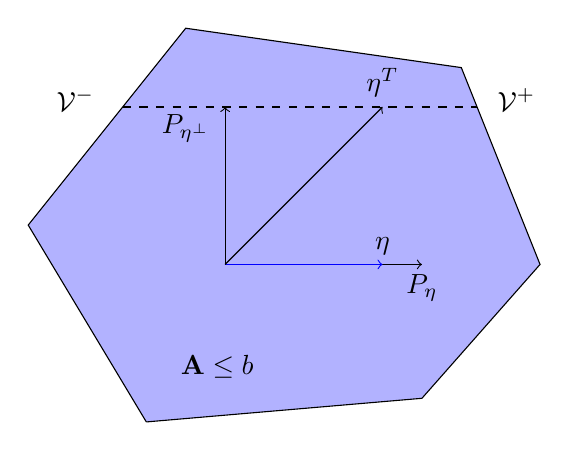
\begin{tikzpicture}
\draw (-1,-2) -- (-2.5,0.5) -- (-0.5,3)-- (3,2.5) -- (4,0) -- (2.5,-1.7) -- (-1,-2)[fill = blue!30];
\draw [<-] (0,2) node [label={[xshift=-0.5cm, yshift=-0.7cm]$P_{\boldsymbol{\eta}^\perp} \y$}] {} -- (0,0);
\draw[<-] (2.5,0) node [below] {$P_{\boldsymbol{\eta}} \y$} -- (0,0);
\draw[<-][blue] (2,0) node [black, above] {$\boldsymbol{\eta}$} -- (0,0);
\draw[<-] (2,2) node [above] {$\boldsymbol{\eta}^T \y$} -- (0,0) node [label={[xshift=1.7cm, yshift=1cm]$\y$}] {};
\draw[dashed] (-1.3,2) node [label={[xshift=-0.6cm, yshift=-0.3cm]$\mathcal{V}^- \del{\y}$}] {} -- (3.2,2) node [label={[xshift=0.5cm, yshift=-0.3cm]$\mathcal{V}^+ \del{\y}$}] {};
\draw node [label={[xshift=-0.1cm, yshift=-1.7cm]$\cbr{\mathbf{A} \y \leq b}$}] {};
\end{tikzpicture}
%\item h
 \end{columns}
% 
% \begin{columns}[t]
%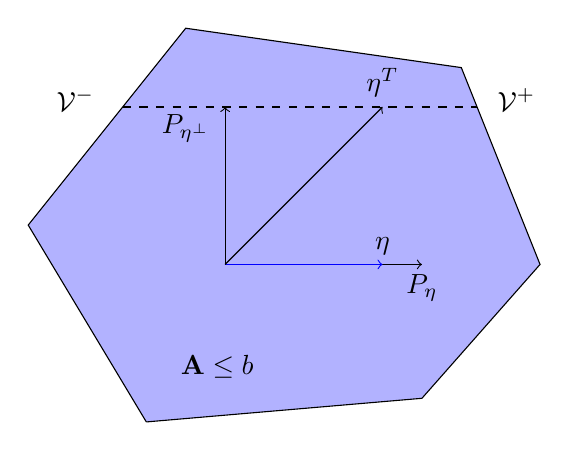
\begin{tikzpicture}
\draw (-1,-2) -- (-2.5,0.5) -- (-0.5,3)-- (3,2.5) -- (4,0) -- (2.5,-1.7) -- (-1,-2)[fill = blue!30];
\draw [<-] (0,2) node [label={[xshift=-0.5cm, yshift=-0.7cm]$P_{\boldsymbol{\eta}^\perp} \y$}] {} -- (0,0);
\draw[<-] (2.5,0) node [below] {$P_{\boldsymbol{\eta}} \y$} -- (0,0);
\draw[<-][blue] (2,0) node [black, above] {$\boldsymbol{\eta}$} -- (0,0);
\draw[<-] (2,2) node [above] {$\boldsymbol{\eta}^T \y$} -- (0,0) node [label={[xshift=1.7cm, yshift=1cm]$\y$}] {};
\draw[dashed] (-1.3,2) node [label={[xshift=-0.6cm, yshift=-0.3cm]$\mathcal{V}^- \del{\y}$}] {} -- (3.2,2) node [label={[xshift=0.5cm, yshift=-0.3cm]$\mathcal{V}^+ \del{\y}$}] {};
\draw node [label={[xshift=-0.1cm, yshift=-1.7cm]$\cbr{\mathbf{A} \y \leq b}$}] {};
\end{tikzpicture}
% \end{columns}
\end{frame}

\begin{frame}{Statistisk inferens}{Polyeder lemma}
\begin{itemize}
\item Af polyede lemmaet kan fordeling af enhver lineær funktion $\boldsymbol \eta^T \vy$ givet $\boldsymbol \Gamma \vy \geq u$ skrives som en følgende betinget fordeling
\begin{align*}
\boldsymbol \eta^T \vy \given \pazocal{V}^- \del{\vy} \leq \boldsymbol \eta^T \vy \leq \pazocal{V}^+ \del{\vy}.
\end{align*}
Da $\boldsymbol \eta^T \vy $ er normalfordeling, er overstående trunkeret normalfordelt. 
\end{itemize}
\end{frame}

\begin{frame}{Statistisk inferens}{Polyeder lemma}
\begin{block}{Lemma}
Lad \(\Phi \del{x}\) betegne fordelingsfunktionen af en standard normalfordeling, da er fordelingsfunktionen af en trunkeret normalfordelt stokastisk variabel med middelværdi \(\mu\) og varians \(\sigma^2\) indenfor intervallet \(\sbr{a,b}\) givet ved
\begin{align*}
F_{\mu, \sigma^2}^{\sbr{a,b}} \del{x} = \frac{\Phi\del{\frac{x-\mu}{\sigma}} - \Phi\del{\frac{a-\mu}{\sigma}}}{\Phi\del{\frac{b-\mu}{\sigma}} - \Phi\del{\frac{a-\mu}{\sigma}}}.
\end{align*}
Hvis \(\boldsymbol{\eta}^T \boldsymbol{\Sigma} \boldsymbol{\eta} \neq 0\), da er 
\begin{align*}
F_{\boldsymbol{\eta}^T \vmu, \boldsymbol{\eta}^T \boldsymbol{\Sigma} \boldsymbol{\eta}}^{\sbr{\pazocal{V}^-,\pazocal{V}^+}} \del{\boldsymbol{\eta}^T \vy} \given  \boldsymbol{\Gamma} \vy \geq \mathbf{u} \sim Unif(0,1)
\end{align*}
\end{block}
\end{frame}

\begin{frame}{Statistisk inferens}{Polyeder lemma}
\begin{itemize}
\item Overstående lemma anvendes til at lave betinget inferens af enhver lineær funktion $\boldsymbol \eta^T \vy $ . Vi kan udregne $p$-værdier for nulhypotesen  $\pazocal{H}_0:\boldsymbol \eta^T \vmu  = 0$ og tilhørende betingede konfidensintervaller
\end{itemize}
\end{frame}

\begin{frame}{Statistisk inferens}{TG testen}
\begin{block}{TG testen}
\begin{itemize}
%\item Vi har, at $\boldsymbol \eta^T \vy \sim N\del{\boldsymbol \eta^T \vmu , \sigma^2 \Vert \boldsymbol \eta \Vert^2_2}$ i intervallet $[\pazocal{V}^-, \pazocal{V}^+ ]$
\item Antager at $\vX$ er i general position
\item Vi laver inferens om $ \boldsymbol \eta^T \vmu \given \boldsymbol \Gamma \vy \geq 0 $
\begin{align*}
 \pazocal{H}_0 : \boldsymbol \eta^T \vmu = 0 \quad \text{imod} \quad  \pazocal{H}_1 : \boldsymbol \eta^T \vmu  \neq 0
\end{align*}
\item Teststørrelsen er givet ved
\begin{align*}
T_k^{TG} = 2 \min \cbr{T_k^{tg}, 1 - T_k^{tg} } 
\end{align*}
og er standard uniform fordelt, hvor 
\begin{align*}
T_k^{tg} & = 1 - F_{0, \sigma^2 \Vert \boldsymbol \eta \Vert^2_2}^{[\pazocal{V}^-, \pazocal{V}^+ ]} \del{\boldsymbol \eta^T \vy} \\
%\pazocal{V}^- \del{\vy} & = \underset{j:\del{\boldsymbol \Gamma \boldsymbol \eta}_j >0}{\max} - \del{\boldsymbol \Gamma \vy}_j \cdot \frac{\Vert \boldsymbol \eta \Vert^2_2}{\del{\boldsymbol \Gamma \boldsymbol \eta}_j} + \boldsymbol \eta^T \vy \\
%\pazocal{V}^+ \del{\vy} & =  \underset{j:\del{\boldsymbol \Gamma \boldsymbol \eta}_j <0}{\max} - \del{\boldsymbol \Gamma \vy}_j \cdot \frac{\Vert \boldsymbol \eta \Vert^2_2}{\del{\boldsymbol \Gamma \boldsymbol \eta}_j} + \boldsymbol \eta^T \vy  
\end{align*}

\end{itemize}
\end{block}
\end{frame}

